\documentclass[a4paper]{article}

\usepackage[english]{babel}
\usepackage[utf8]{inputenc}
\usepackage{amsmath}
\usepackage{graphicx}
\usepackage[colorinlistoftodos]{todonotes}

\begin{document}

\begin{figure}
\centering
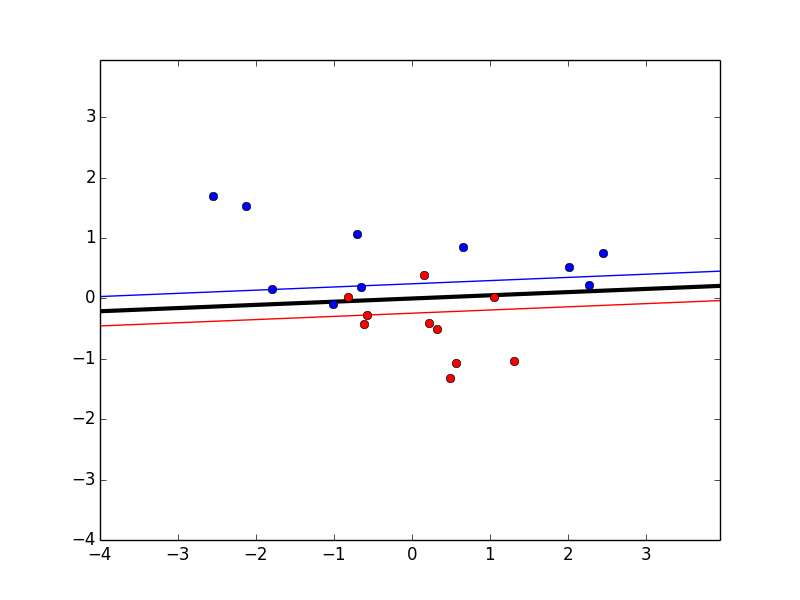
\includegraphics[width=0.8\textwidth]{linear_kernel.png}
\caption{\label{fig:linear_kernel}Linear kernel}
\end{figure}

\begin{figure}
\centering
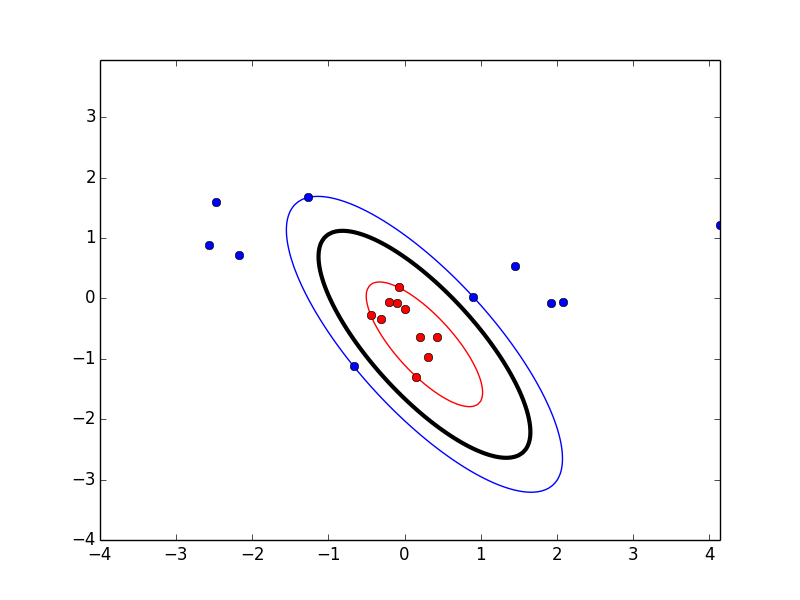
\includegraphics[width=0.8\textwidth]{polynomial_kernel_2.png}
\caption{\label{fig:polynomial_kernel_2}Polynomial kernel, p = 2}
\end{figure}

\begin{figure}
\centering
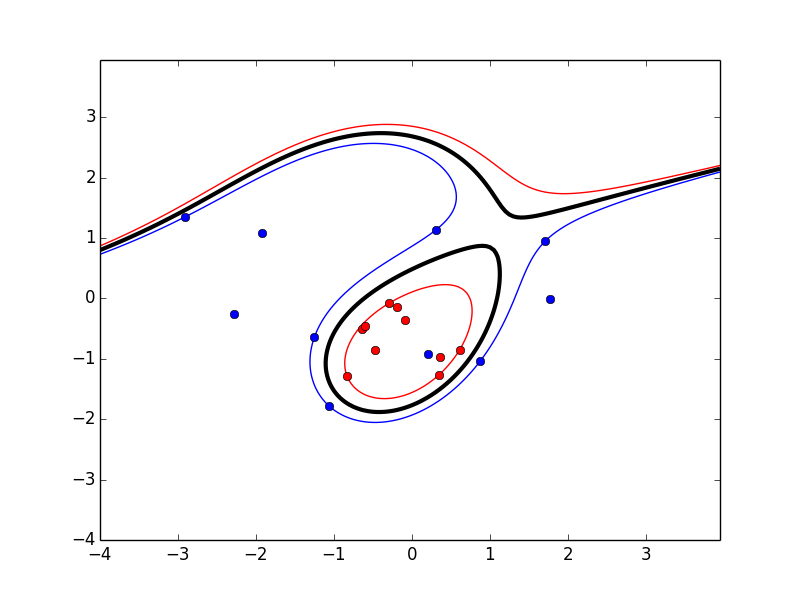
\includegraphics[width=0.8\textwidth]{polynomial_kernel_3.png}
\caption{\label{fig:polynomial_kernel_3}Polynomial kernel, p = 3}
\end{figure}

\begin{figure}
\centering
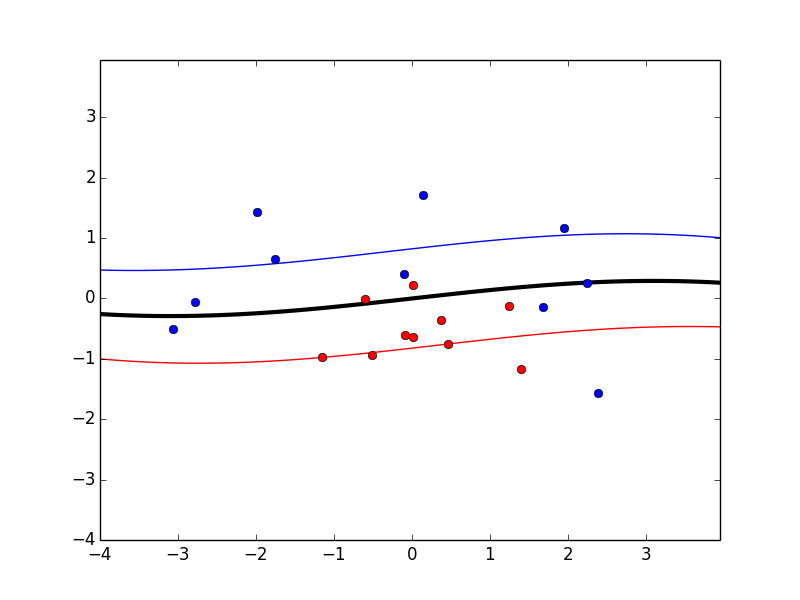
\includegraphics[width=0.8\textwidth]{sigmoid_kernel.png}
\caption{\label{fig:sigmoid_kernel}Sigmoid kernel}
\end{figure}

\begin{figure}
\centering
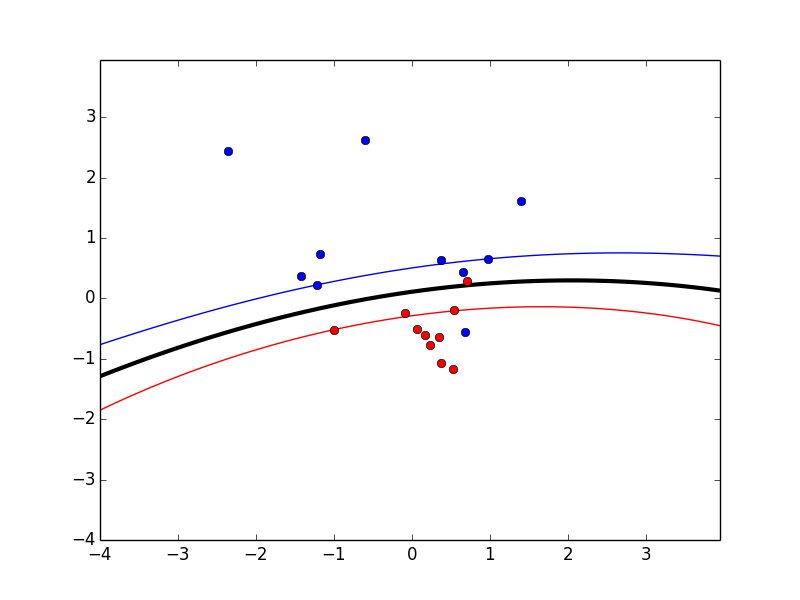
\includegraphics[width=0.8\textwidth]{rbf_kernel.png}
\caption{\label{fig:rbf_kernel}Radial basis function kernel}
\end{figure}

\end{document}